\documentclass[]{mwart}

\usepackage{polski}
\usepackage[utf8]{inputenc}

\usepackage{amsthm}
\usepackage{amsmath}
\usepackage{amssymb}

\usepackage{mdframed}
\usepackage{hyperref}
\usepackage[%draft%      % dla obrazkow zakomentowac draft
]{graphicx}  
\usepackage{url}
\usepackage{enumitem}
\usepackage{verbatim}
\usepackage{caption}


    
\usepackage{float}      



\usepackage{fancyhdr}
\pagestyle{fancy}
\fancyhf{}

\fancyhead[L]{
\includegraphics[height=0.666cm]{wspolne_dla_wszystkich/logo_projektu.png}}
\fancyhead[C]{\textit{Poprawa jakości zdjęć}}
\fancyhead[R]{
\includegraphics[height=0.9cm]{wspolne_dla_wszystkich/logo_uczelni.png}}
\fancyfoot[C]{\thepage}

\setlength{\headheight}{20pt}  



\usepackage{listings}
\usepackage{xcolor} 




\begin{document}
\thispagestyle{empty}

\begin{figure}[h]
    \centering
    
\includegraphics[width=1\textwidth]{wspolne_dla_wszystkich/logo_uczelni.png}
\end{figure}


\begin{center}
    {\LARGE \textbf{Poprawa jakości skanów zdjęć wykonanych techniką analogową
        }} \\[0.3cm]
    {\large \textbf{Raport II}} \\[0.2cm]
    \textit{projekt realizowany pod opieką prof. dr hab. inż. Artura Przelaskowskiego}

\end{center}

\begin{figure}[h]
    \centering
    
\includegraphics[width=1\textwidth]{wspolne_dla_wszystkich/logo_projektu.png}
\end{figure}

\vfill
\begin{abstract}
    Raport 3 projektu poprawy jakości cyfrowych skanów zdjęć wykonanych techniką analogową przez grupę nr 9 (wtorkową z godziny 18)
    w składzie:  Bartosz Wójcik, Katarzyna Szwed, Natalia Szymańska,
    Patrycja Szałajko, Aleksandra Wójcik, Karol Sęk, Michał Juszkiewicz, Filip Sajko.

    W tym raporcie opiszemy nasze działania prowadzące do poprawy działania programu i opiszemy poprawki.
    Zajmiemy się ponadto ekstensywnym testowaniem działania naszego programu i wyciągnięciem wniosków na temat jego działania i optymalnych ustawień.
\end{abstract}

\newpage
\tableofcontents{}

\newpage

% ADD KOREKTA
\section{Korekta do raportu 2}
\begin{itemize}
    \item Dla zdjęcia dziewczyny z poprzedniego raportu szerokość filtru gaussowskiego $ =  37/71$.
\end{itemize}


\section{Rozszerzanie działalności programu}
\subsection{Słowem wstępu...}
Głównym celem naszego programu jest coś, co można nazwać
ogólnie (konkretnie nasz cel zdefiniowaliśmy w poprzednim raporcie)
poprawą jakości skanów zdjęć analogowych. Trzeba jednak pamiętać,
że najważniejszym ogniwem każdego problemu jest człowiek, którego
problem ten dotyczy -- i któremu chce się pomóc oferując dane rozwiązania. \newline

Tak więc łatwo zauważyć, że kluczowym elementem każdego programu jest dobrze wykonany
interfejs użytkownika. W ostatecznym rozrachunku przecież gorszy
jest przecież program z najlepszym algorytmem, ale złym interfejsem, z którego użytkownik i tak nie skorzysta. \newline

% program z nawet najlepszym algorytmem skrytym pod płaszczem źle zaprojektowanego,
% nieczytelnego i nieprzyjaznego interfejsu od którego użytkownik się odbije
% i koniec końców z usług którego nie skorzysta. \newline

Rozumiejąc tę potrzebę wraz z optymalizacją i rozszerzaniem funkcjonalności
naszego programu, stworzyliśmy interfejs użytkownika i zaczęliśmy % tja... na pewno
tworzyć szczegółową instrukcję obsługi naszego programu.

\subsection{Menu programu}
Na chwilę obecną główne menu naszego programu oferuje następujące opcje:

\begin{table}[h]
    \centering
    \begin{tabular}{|c|l|}
        \hline
        Lp. & Opcja                                 \\ \hline
        1   & usuwanie farfocli                     \\ \hline       %
        2   & normalizacja histogramu jasności      \\ \hline       %
        3   & filtracja filtrem bilateralnym        \\ \hline       %
        4   & filtracja filtrem gaussowskim         \\ \hline       %
        5   & usuwanie szumu -- uśrednianie pikseli \\ \hline       %
        6   & wyostrzenie -- maska wyostrzająca     \\ \hline       %
    \end{tabular}
    \caption{Opcje główne naszego programu dostępne dla użytkownika}
\end{table}

Teraz zajmiemy się szczegółowym omówieniem wymienionych w powyżej tabeli opcji. \newpage






\section{Usuwanie farfocli}

\subsection{Słowem wstępu}
Jest to główny cel naszego projektu i problem z którym się mierzyliśmy podczas poprzedniego etapu.

Szczegółowo sposób wykrywania, usuwania tego typu artefaktów i normalizowania
zdjęć nimi zanieczyszczonych opisaliśmy w poprzednim raporcie.

W tej części chcielibyśmy zająć się głównie opisaniem efektów naszej pracy.

\subsection{Efekty ogólne i ciekawe przypadki}
W prawie wszystkich testowanych przez nas przypadkach działanie programu w sposób widoczny poprawiało jakość i estetykę zdjęcia.

Co ciekawe, podczas naszych testów odkryliśmy, że ta nasza funkcjonalność
wyjątkowo dobrze sobie z usuwaniem nacieków i zarysowań na znajdujących się na zdjęciach:

\newpage

\begin{figure}[H]
    \centering
    \includegraphics[width=\linewidth, keepaspectratio]{Photos2/przed/gpt1.png}
    \caption{Zdjęcie dziewczyny z wyraźnymi farfoclami.}
\end{figure}
\begin{figure}[H]
    \centering
    \includegraphics[width=\linewidth, keepaspectratio]{Photos2/po/gpt1.png}
    \caption{Zdjęcie poprawione, szerokość filtru gaussowskiego $37/71$.}
\end{figure}

\begin{figure}[H]
    \centering
    \includegraphics[width=\linewidth, keepaspectratio]{Photos3/1 farfocle/pogrzeb_before.png}
    \caption{Zdjęcie zarysowane.}
\end{figure}
\begin{figure}[H]
    \centering
    \includegraphics[width=\linewidth, keepaspectratio]{Photos3/1 farfocle/pogrzeb_after.png}
    \caption{Zdjęcie poprawione, szerokość filtru gaussowskiego $29/71$.}
\end{figure}

\begin{figure}[H]
    \centering
    \includegraphics[width=\linewidth, keepaspectratio]{Photos3/1 farfocle/dziewczyna_before.jpg}
    \caption{Zdjęcie z zaciekami.}
\end{figure}
\begin{figure}[H]
    \centering
    \includegraphics[width=\linewidth, keepaspectratio]{Photos3/1 farfocle/dziewczyna_after.jpg}
    \caption{Poprawione zdjęcie, szerokość filtru gaussowskiego $3/71$.}
\end{figure}

\begin{figure}[H]
    \centering
    \includegraphics[width=\linewidth, keepaspectratio]{Photos3/1 farfocle/farfocle4_before.jpg}
    \caption{Zdjęcie z zaciekami.}
\end{figure}
\begin{figure}[H]
    \centering
    \includegraphics[width=\linewidth, keepaspectratio]{Photos3/1 farfocle/farfocle4_after.jpg}
    \caption{Zdjęcie poprawione, szerokość filtru gaussowskiego $3/71$.}
\end{figure}




\newpage

\section{Normalizacja histogramu jasności       }
\subsection{Metoda}
Wyrównanie histogramu jasności jest metodą przetwarzania obrazów, polegającą na
poprawianiu kontrastu zdjęcia z wykorzystaniem jego histogramu -- który się normalizuje.
Metoda ta rozciąga wartości pikseli z obrazu na cały przedział jasności.
Dzięki temu, fragmenty zdjęcia o pierwotnie niskim poziomie kontrastu stają się czytelniejsze.

\subsection{Przykłady}
Metoda ta jest bardzo skuteczna w poprawianiu kontrastu zdjęcia -- niestety czasem
kosztem jakości zdjęcia. Metoda ta nie rozróżnia sygnału od szumu co może spowodować wzrost wartości szumu,
przy jednoczesnym zmniejszeniu widoczności właściwego sygnału -- co widać na poniższym zdjęciu.


\begin{figure}[H]
    \centering
    \includegraphics[width=\linewidth, keepaspectratio]{Photos3/normalizacja histogramu/test2m.PNG}
    \caption{Zdjęcie przed normalizacją wraz z histogramem.}
\end{figure}
\begin{figure}[H]
    \centering
    \includegraphics[width=\linewidth, keepaspectratio]{Photos3/normalizacja histogramu/test2cm.PNG}
    \caption{Zdjęcie po normalizacji (zaszumione) wraz z histogramem.}
\end{figure}

\newpage

\begin{figure}[H]
    \centering
    \includegraphics[width=\linewidth, keepaspectratio]{Photos3/2 normalizacja histogramu jasności/hist/motor_intensity.jpg}
    \caption{Zdjęcie przed normalizacją wraz z histogramem.}
\end{figure}
\begin{figure}[H]
    \centering
    \includegraphics[width=\linewidth, keepaspectratio]{Photos3/2 normalizacja histogramu jasności/hist/motor_after_intensity.jpg}
    \caption{Zdjęcie po normalizacji wraz z histogramem.}
\end{figure}

% \begin{figure}[H]
%     \centering
%     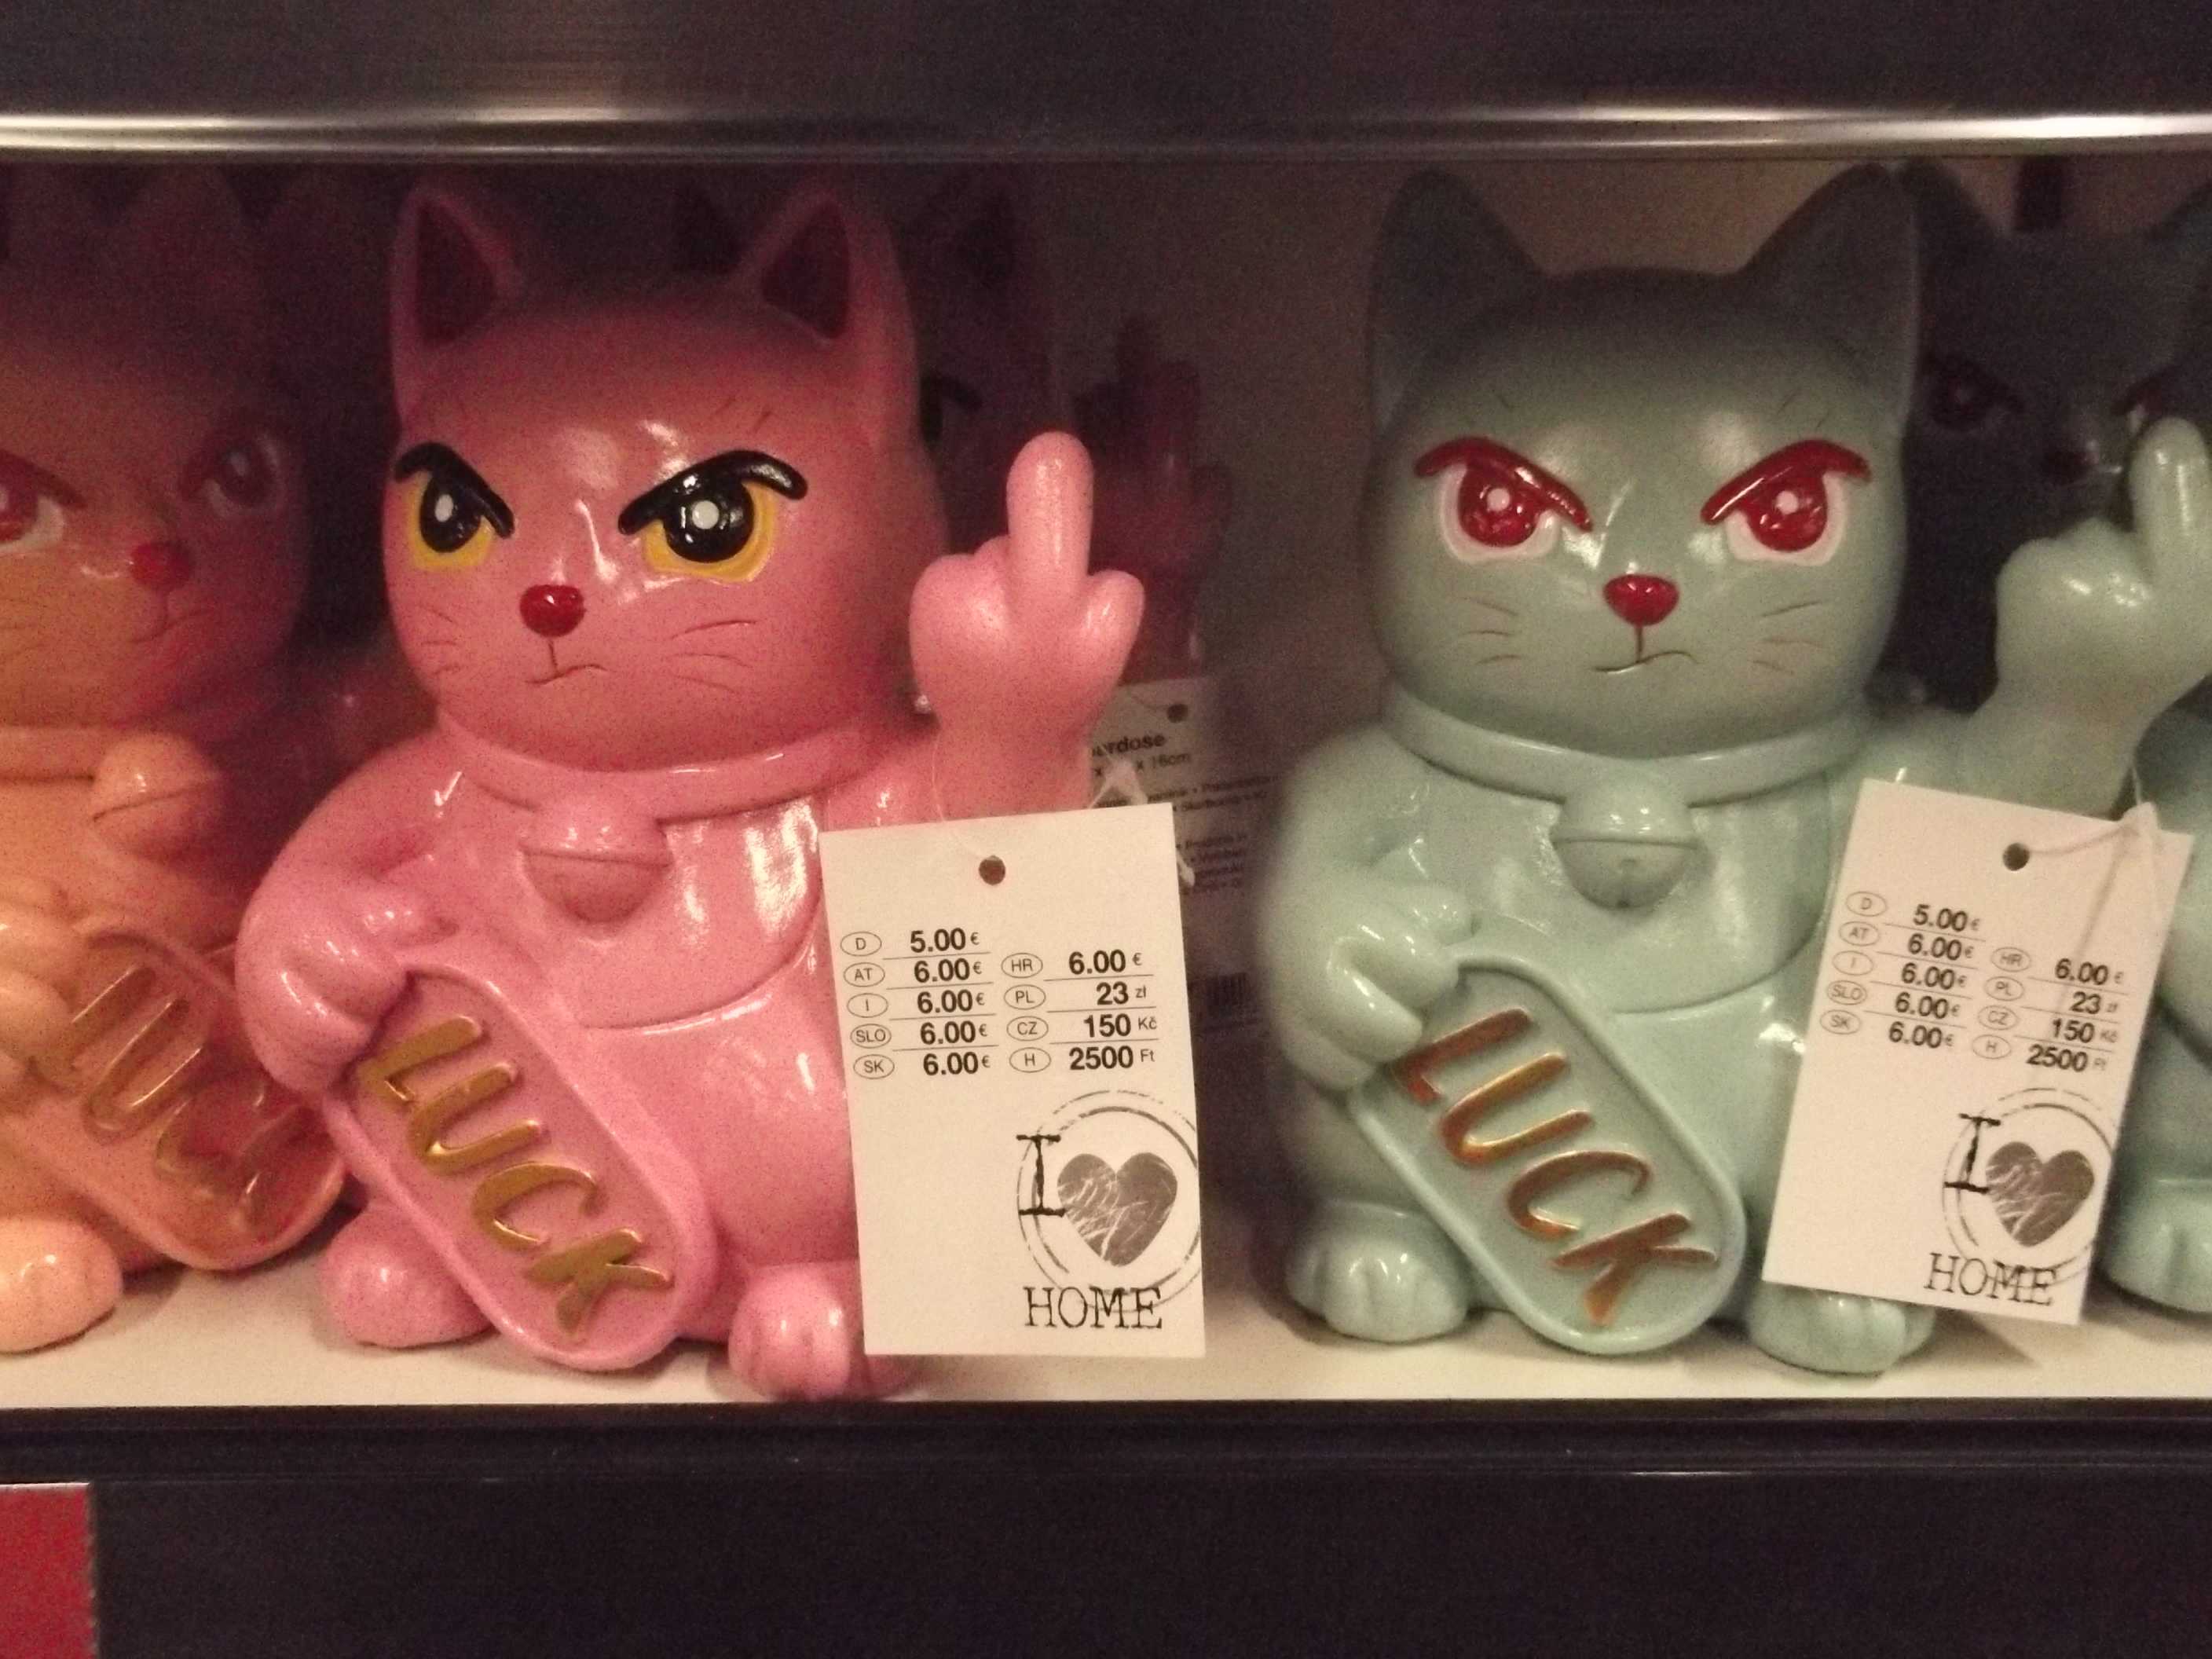
\includegraphics[width=\linewidth, keepaspectratio]{Photos3/2 normalizacja histogramu jasności/before/kot2.jpg}
%     \caption{Zdjęcie przed normalizacją wraz z histogramem.}
% \end{figure}
% \begin{figure}[H]
%     \centering
%     \includegraphics[width=\linewidth, keepaspectratio]{Photos3/2 normalizacja histogramu jasności/after/kot2_after.jpg}
%     \caption{Zdjęcie po normalizacji (zaszumione) wraz z histogramem.}
% \end{figure}



\vfill
\section{Filtracja filtrem bilateralnym         }
\subsection{Metoda}
Filtr bilateralny jest nieliniowym filtrem wygładzającym, przede wszystkim charakteryzuje się tym,
że zachowuje krawędzie i redukuje szum.

Zastępuje on intensywność każdego piksela średnią ważoną intensywności pobliskich pikseli
wyliczoną poprzez filtr o odpowiednim rozmiarze.
Jeżeli wartość danego piksela jest bliska wartości piksela w centrum filtru, jego waga jest --
oparta na rozkładzie Gaussa. W przeciwnym wypadku waga jest bliska 0.
Ta złożona zależność pozwala zachować ostre krawędzie przy jednoczesnym tłumieniu szumu. \newpage

\subsection{Przykłady}

\begin{figure}[H]
    \centering
    \includegraphics[angle=90, width=\linewidth, keepaspectratio]{Photos3/filtr bilateralny/test3.jpg}
    \caption{Zdjęcie pierwotne.}
\end{figure} \newpage
\begin{figure}[H]
    \centering
    \includegraphics[width=\linewidth, keepaspectratio]{Photos3/filtr bilateralny/test3b.jpg}
    \caption{Zdjęcie po zastosowaniu filtru bilateralnego.}
\end{figure}






\section{Filtracja filtrem gaussowskim           }
\subsection{O rozmyciu gaussowskim}
Filtracja filtrem gaussowskim oparta jest na generowaniu maski poprzez tworzenie rozmycia gaussowskiego zdjęcia.

Wygładzanie gaussowskie jest efektem rozmywania obrazu za pomocą funkcji rozkładu Gaussa,
która jest szeroko wykorzystywana w grafice komputerowej w celu uzyskania wygładzenia obrazu i wyciszenia szumu informacyjnego.

Wygładzenie paradoksalnie pomimo utraty ostrości obrazu przyczynia się do poprawy wizualnego odbioru zdjęcia.

\subsection{Przykłady}
% probably złe zdjęcia -- praca domowa dla Karola.

\begin{figure}[H]
    \centering
    \includegraphics[angle=90, width=\linewidth, keepaspectratio]{Photos3/filtr gaussowski/test3.jpg}
    \caption{Zdjęcie przed.}
\end{figure} \newpage
\begin{figure}[H]
    \centering
    \includegraphics[width=\linewidth, keepaspectratio]{Photos3/filtr gaussowski/test3g.jpg}
    \caption{Zdjęcie po.}
\end{figure}





\vfill
\section{Usuwaniem szumu -- uśrednianie pikseli}
\subsection{Metoda}
Ta metoda polega na uśrednianiu wartości pikseli w oparciu o piksele do nich podobne.

Dane piksele uznaje się za podobne, jeśli średnia jasność ich otoczenia
jest zbliżona. Następnie, wartość danego piksela jest zastępowana
średnią wartością wszystkich pikseli podobnych do niego.

W przeciwieństwie do innych metod usuwania szumu, metoda ta nie jest lokalna,
dla każdego piksela piksele podobne mogą się znajdować gdziekolwiek na zdjęciu.

Algorytm ten usuwa szum nie niszcząc struktury i detali zdjęcia, jednakże
czasami okazuje się mieć nieznaczne efekty. \newpage

\subsection{Przykłady}
\begin{figure}[H]
    \centering
    \includegraphics[width=\linewidth, keepaspectratio]{Photos3/5 szum/srodmiescie_before_szum.jpg}
    \caption{Zdjęcie przed usuwaniem szumu.}
\end{figure}
\begin{figure}[H]
    \centering
    \includegraphics[width=\linewidth, keepaspectratio]{Photos3/5 szum/srodmiescie_after_szum.jpg}
    \caption{Zdjęcie po usuwaniu szumu.}
\end{figure} \newpage

\begin{figure}[H]
    \centering
    \includegraphics[width=\linewidth, keepaspectratio]{Photos3/5 szum/motor_before_szum.jpg}
    \caption{Zdjęcie przed usuwaniem szumu.}
\end{figure}
\begin{figure}[H]
    \centering
    \includegraphics[width=\linewidth, keepaspectratio]{Photos3/5 szum/motor_after_szum.jpg}
    \caption{Zdjęcie po usuwaniu szumu.}
\end{figure}

\begin{figure}[H]
    \centering
    \includegraphics[width=\linewidth, keepaspectratio]{Photos3/6 wyostrzanie maską wyostrzającą/pogrzeb_ostrosc.png}
    \caption{Zdjęcie przed usuwaniem szumu.}
\end{figure}
\begin{figure}[H]
    \centering
    \includegraphics[width=\linewidth, keepaspectratio]{Photos3/6 wyostrzanie maską wyostrzającą/pogrzeb_odszum.png}
    \caption{Zdjęcie po usuwaniu szumu.}
\end{figure}



\newpage
\section{Wyostrzenie -- maska wyostrzająca      }

\subsection{Metoda}
Wyostrzanie za pomocą maski nieostrości jest techniką wyostrzania obrazu
powszechnie wykorzystywaną w obróbce fotografii w celu poprawy ostrości zdjęć.

Nazwa pochodzi od faktu, że technika ta wykorzystuje rozmyty,
`nieostry' negatyw obrazu do stworzenia maski obrazu oryginalnego.
Maska nieostra jest następnie łączona z oryginalnym pozytywem,
tworząc obraz mniej rozmyty niż pierwotny. Uzyskany obraz mimo, że wyraźniejszy
może okazać się mniej wiernym odwzorowaniem oryginalnego obrazu.

\subsection{Przykłady}
\begin{figure}[H]
    \centering
    \includegraphics[width=\linewidth, keepaspectratio]{Photos3/6 wyostrzanie maską wyostrzającą/dzieci.png}
    \caption{Zdjęcie przed wyostrzeniem maską wyostrzającą.}
\end{figure}
\begin{figure}[H]
    \centering
    \includegraphics[width=\linewidth, keepaspectratio]{Photos3/6 wyostrzanie maską wyostrzającą/dzieci_ostrosc.png}
    \caption{Zdjęcie po wyostrzeniu maską wyostrzającą.}
\end{figure}

\begin{figure}[H]
    \centering
    \includegraphics[angle=-90, width=\linewidth, keepaspectratio]{Photos3/6 wyostrzanie maską wyostrzającą/dziadek.png}
    \caption{Zdjęcie przed wyostrzeniem maską wyostrzającą.}
\end{figure}
\begin{figure}[H]
    \centering
    \includegraphics[angle=-90, width=\linewidth, keepaspectratio]{Photos3/6 wyostrzanie maską wyostrzającą/dziadek_ostrosc.png}
    \caption{Zdjęcie po wyostrzeniu maską wyostrzającą.}
\end{figure}








\newpage
\section{Przykładowe wykorzystanie programu jako całości}
Dzięki naszym badaniom wypracowaliśmy narzędzie o szerokim zastosowaniu w życiu codziennym.
Aby zmaksymalizować jego skuteczność, przeprowadziliśmy dodatkowe badania,
mające na celu ustalenie najefektywniejszej metody użycia. Odkryliśmy, że najlepsze efekty osiągamy,
stosując kolejno narzędzia do usuwania farfocli, poprawiania ostrości oraz odszumiania.

Dzieje się tak dlatego, że najpierw eliminujemy obce elementy,
powstałe jako zanieczyszczenia fizyczne podczas skanowania.
Kolejny etap -- poprawianie ostrości -- zwiększa jednak poziom szumu,
dlatego końcowe odszumianie cofa niepożądane skutki uboczne poprzedniego kroku.

Trzeba jednak podkreślić, że nasze narzędzie nie jest na tym etapie w pełni zautomatyzowane
-- każde zdjęcie wymaga indywidualnej obróbki, dostosowanej do specyfiki problemu.
Widać to, analizując fotografie użyte w badaniach: w zależności od potrzeb stosowaliśmy różne maski,
które dopasowywaliśmy do konkretnej sytuacji.




\section{Dostępność programu}
Na chwilę obecną nasze rozwiązanie jest zaawansowanym programem terminalowym,
działającym na każdym systemie z dostępną i zainstalowaną biblioteką OpenCV oraz
dowolnym kompilatorem języka C++ zdolnym do kompilacji na tym systemie lub jego pochodnym.

Program dostępny jest na licencji \textit{open source} i jego kod źródłowy można znaleźć na GitHubie
pod adresem:
\begin{center}
    \url{https://github.com/ssk12o/PTI-Foto-Projekt}.
\end{center}
skąd można go łatwo pobrać, skompilować i wykorzystywać dowolnie (choć zgodnie z przeznaczeniem!).




\newpage
\section{Wykorzystywane narzędzia}
W tej części naszego projektu korzystaliśmy z następujących narzędzi:
\begin{itemize}
    \item Programu i języka Matlab -- do analizy zdjęć;
    \item Języka C++ -- do napisania programu usuwającego artefakty;
    \item Programu VS Code -- do tworzenia, edycji i dokumentacji kodu programu i raportów;
    \item Programu LibreOffice Calc -- do analizy części danych numerycznych;
    \item $\LaTeXe{}$ -- do przygotowania raportu;
    \item Strony Github i programu Git -- do udostępniania, dystrybucji i pracy nad kodem;
    \item 7zip -- do kompresji zdjęć;
    \item Google Drive -- do udostępniania części dużych plików;
    \item Skanera minilab Noritsu HS-1800 -- do w dalszej części wykonywania wysokiej jakości cyfrowych skanów zdjęć wykonanych techniką analogową;
    \item Aparatów:
          \begin{itemize}
              \item Canon EOS 300 z obiektywem Tamron 28-105mm 1:4-5.6 i kliszą Fomapan 400
              \item Fujifilm FinePix L55 Digital Camera -- Black (12MP, 3x Optical Zoom)
          \end{itemize}
\end{itemize}


\section{Podział obowiązków}
Na tym etapie projektu podzieliśmy się pracą, obowiązkami i zadaniami w następujący sposób:
\begin{itemize}
    \item Bartosz Wójcik -- wykonywanie, skanowanie i analiza zdjęć; research.
    \item Katarzyna Szwed -- korekta raportu; analiza zdjęć i działania programu.
    \item Natalia Szymańska -- pisanie raportu.
    \item Patrycja Szałajko -- zarządzanie pracą zespołu, kontakt.
    \item Aleksandra Wójcik -- skanowanie zdjęć rodzinnych w celu polepszenia ich jakości w końcowych etapach projektu.
    \item Karol Sęk -- tworzenie, analizowanie i pisanie algorytmu.
    \item Michał Juszkiewicz -- tworzenie, analizowanie i pisanie algorytmu.
    \item Filip Sajko -- pisanie raportu, implementacja w \LaTeXe{}.
\end{itemize}





%                       Wersja alternatywna podziału obowiązków
% \section{Podział obowiązków}
% Na tym etapie projektu podzieliśmy się pracą, obowiązkami i zadaniami w następujący sposób:
% 
% \begin{table}[h!]
%     \centering
%     \renewcommand{\arraystretch}{1.3}
%     \begin{tabular}{|p{3cm}|p{7.5cm}|} \hline
%         \textbf{Imię i nazwisko} & \textbf{Zakres obowiązków}                                                               \\ \hline \hline
%         Bartosz Wójcik           & Wykonywanie, skanowanie i analiza zdjęć; opieka merytoryczna.                            \\ \hline
%         Katarzyna Szwed          & Tworzenie, analizowanie i pisanie algorytmu; korekta raportu.                            \\ \hline
%         Natalia Szymańska        & Pisanie raportu.                                                                         \\ \hline
%         Patrycja Szałajko        & Zarządzanie pracą zespołu, kontakt z mediami.                                            \\ \hline
%         Aleksandra Wójcik        & Skanowanie zdjęć rodzinnych w celu polepszenia ich jakości w końcowych etapach projektu. \\ \hline
%         Karol Sęk                & Tworzenie, analizowanie i pisanie algorytmu.                                             \\ \hline
%         Michał Juszkiewicz       & Tworzenie, analizowanie i pisanie algorytmu.                                             \\ \hline
%         Filip Sajko              & Pisanie raportu, implementacja w \LaTeX{}.                                               \\ \hline
%     \end{tabular}
%     \caption{Podział obowiązków w zespole projektowym.}
% \end{table}




\end{document}